\documentclass[t]{beamer}
\usetheme[darktitle]{UniversityOfManchester}

\usepackage{sourcesanspro}
\usepackage{sourcecodepro}
\usepackage[binary-units]{siunitx}

% Document properties
\title{An efficient SpiNNaker implementation of the
       Neural~Engineering~Framework}
\author{Andrew Mundy, James Knight,\\Terry Stewart and Steve Furber}

% Document
\begin{document}
  \maketitle

  % Introduction
  % ------------
  % * Neural engineering framework a tool for large-scale cognitive models,
  %   e.g., Spaun.
  % * Spaun simulation took 2.5hr of compute per 1s of simulation
  % * Presenting a novel implementation of the NEF for SpiNNaker that focusses
  %   on scaling
  \begin{frame}[plain]{Neurally implemented cognitive models}

    \begin{columns}[c]
      \begin{column}{.6\textwidth}
        Spaun -- \SI{2.5}{\hour} compute for \SI{1}{\second} simulation
        \begin{itemize}
          \item Scales badly to larger models
          \item No real-world interaction
        \end{itemize}

        \vskip\baselineskip

        SpiNNaker
        \begin{itemize}
          \item Scalable
          \item Real-time
        \end{itemize}

        \vskip\baselineskip

        \textbf{A bad fit?}
        \begin{itemize}
          \item Memory usage
          \begin{itemize}
            \item Loading time
          \end{itemize}
          \item Compute load
          \item Network load
        \end{itemize}
      \end{column}
      \begin{column}{.4\textwidth}
        \centering

        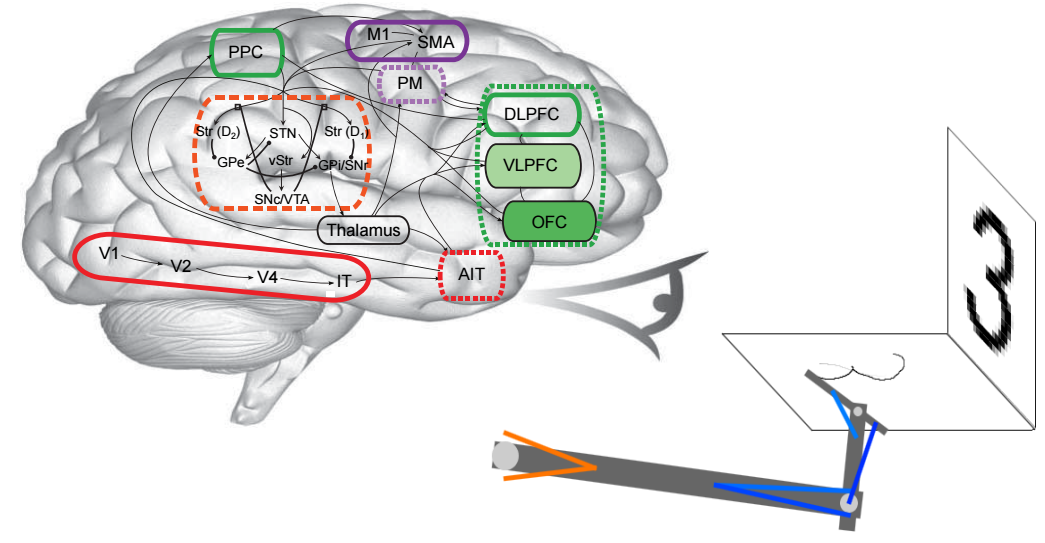
\includegraphics[width=\textwidth]{figures/spaun}

        \vskip2\baselineskip

        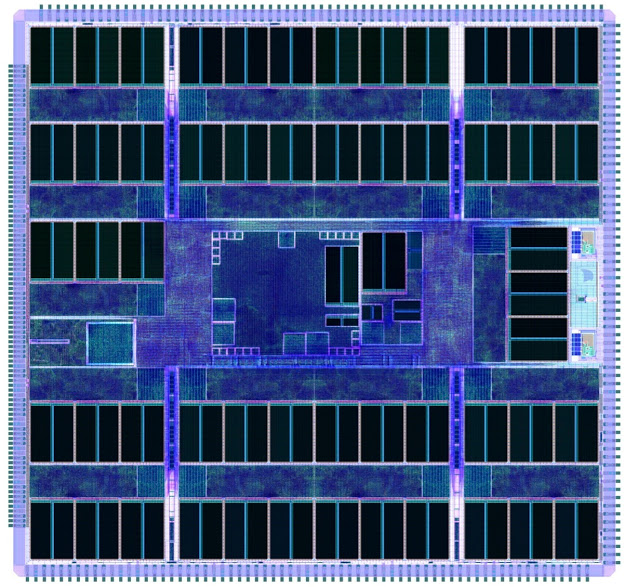
\includegraphics[width=.75\textwidth]{figures/spinnaker}

      \end{column}
    \end{columns}

  \end{frame}

  % Neural Engineering Framework
  % ----------------------------
  % * Ensembles represent vectors in vector spaces
  % * Use weighted linear decoding to compute functions (including identity
  %   function) of that representation
  % Results in:
  % * Dense weight matrices
  % * High firing weights
  \begin{frame}[plain]{Neural Engineering Framework (NEF)}
    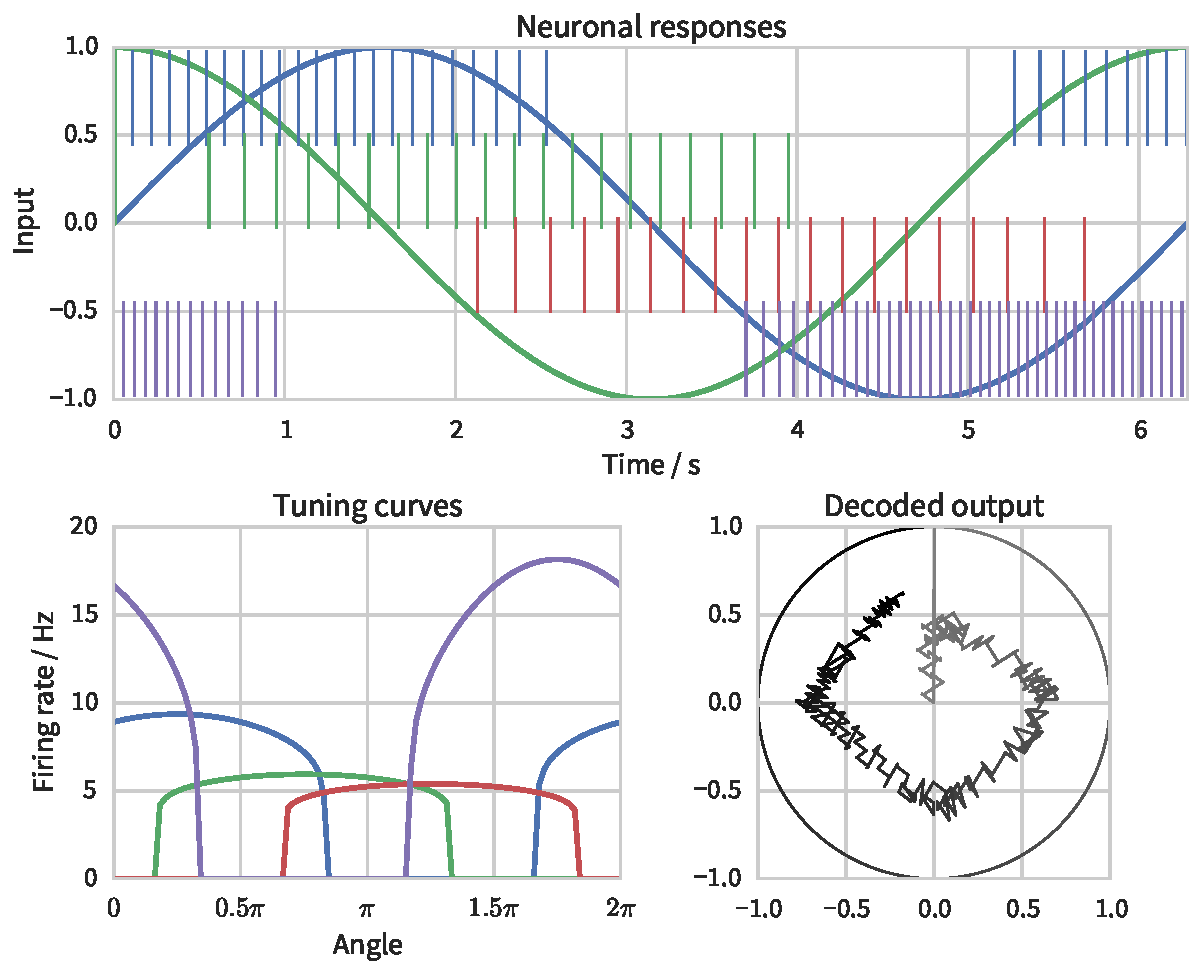
\includegraphics[width=\textwidth]{figures/nef-1}
  \end{frame}

  % SpiNNaker
  % ---------
  % Message passing architecture, event driven
  % Neural net simulation on SpiNNaker:
  % * Deals with individual spikes
  % * Compute constraint: synaptic events
  % * Memory constraint: representing weight matrices
  \begin{frame}{SpiNNaker -- Neural Nets}
    \includegraphics[page=2, width=\textwidth, trim=4.75cm 0 3cm 0, clip]
                    {figures/algorithm_diagram}

    \vskip\baselineskip
    Constrained by
    \begin{description}
      \item[Memory] synaptic weight matrix
      \item[Compute] incoming spike processing
    \end{description}
  \end{frame}

  % Analysis of NEF on SpiNNaker ("Assessing the NEF")
  % --------------------------------------------------
  % * Parameters from Spaun (and general benchmarks) result in poor utilisation
  %   of the architecture
  %    * Memory result for comms channel (~2GiB to represent weight matrices) -
  %      limits to 120 neurons per core
  %    * Event result for comms channel (exceeds synaptic event count for 280
  %      neurons)
  % Result: poor use of the SpiNNaker architecture
  \begin{frame}{Analysis -- NEF on SpiNNaker}

    Using parameters from Spaun
    \begin{itemize}
      \item 512D representational space
      \item 70 neurons per dimension
    \end{itemize}

    \vskip\baselineskip

    Limit of \num{5000} synaptic events per timestep

    \textbf{A 4D communication channel generates \num{5600} events per timestep}

    \vskip\baselineskip

    Each core has \SI{8}{\mebi\byte} memory for weight matrices

    \textbf{One weight-matrix requires \SI{2.28}{\gibi\byte} -- only 120 neurons per core}
  \end{frame}

  % Solution ("Exploiting features of the NEF...")
  % ----------------------------------------------
  % * Explain new algorithm
  \begin{frame}{Efficient SpiNNaker implementation}
    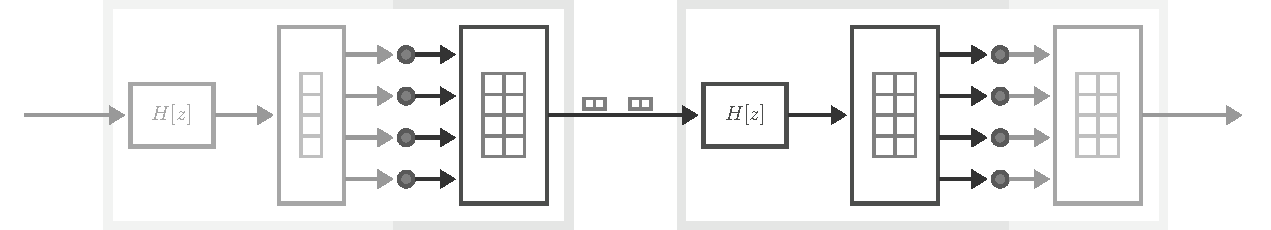
\includegraphics[page=1, width=\textwidth, trim=6.1cm 0 3.75cm 0, clip]
                    {figures/algorithm_diagram}

    \begin{description}
      \item[Less memory] Use factored weight matrices
        \begin{itemize}
          \item Store locally
        \end{itemize}
      \item[Less compute] Represent activity with vectors
        \begin{itemize}
          \item Encoding/decoding cheap
          \item Synaptic filtering in vector-space
        \end{itemize}
    \end{description}
  \end{frame}

  % Results
  % -------
  % * CPU Usage - up to 2000 neurons per core
  % * Memory Usage - 90%+ reductions (with resultant reductions in load time)
  \begin{frame}[plain]{Results -- CPU Usage -- Dimension scaling}
    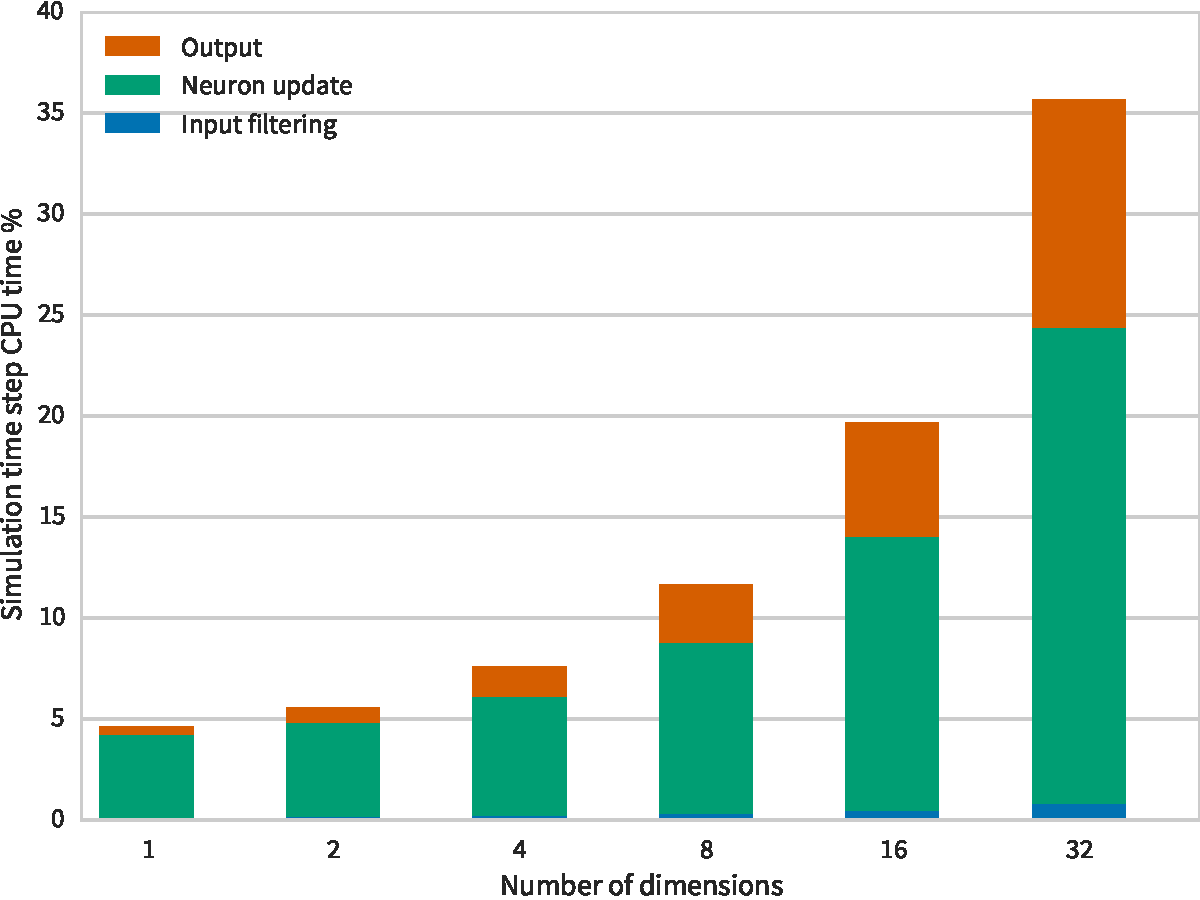
\includegraphics[width=\textwidth]{figures/comm_channel_cpu_100n_bar.pdf}

    {\tiny 100 neurons, \SI{200}{\mega\hertz} clock cycle with
     \SI{1}{\milli\second} simulation step}
  \end{frame}

  \begin{frame}[plain]{Results -- CPU Usage -- Neuron scaling}
    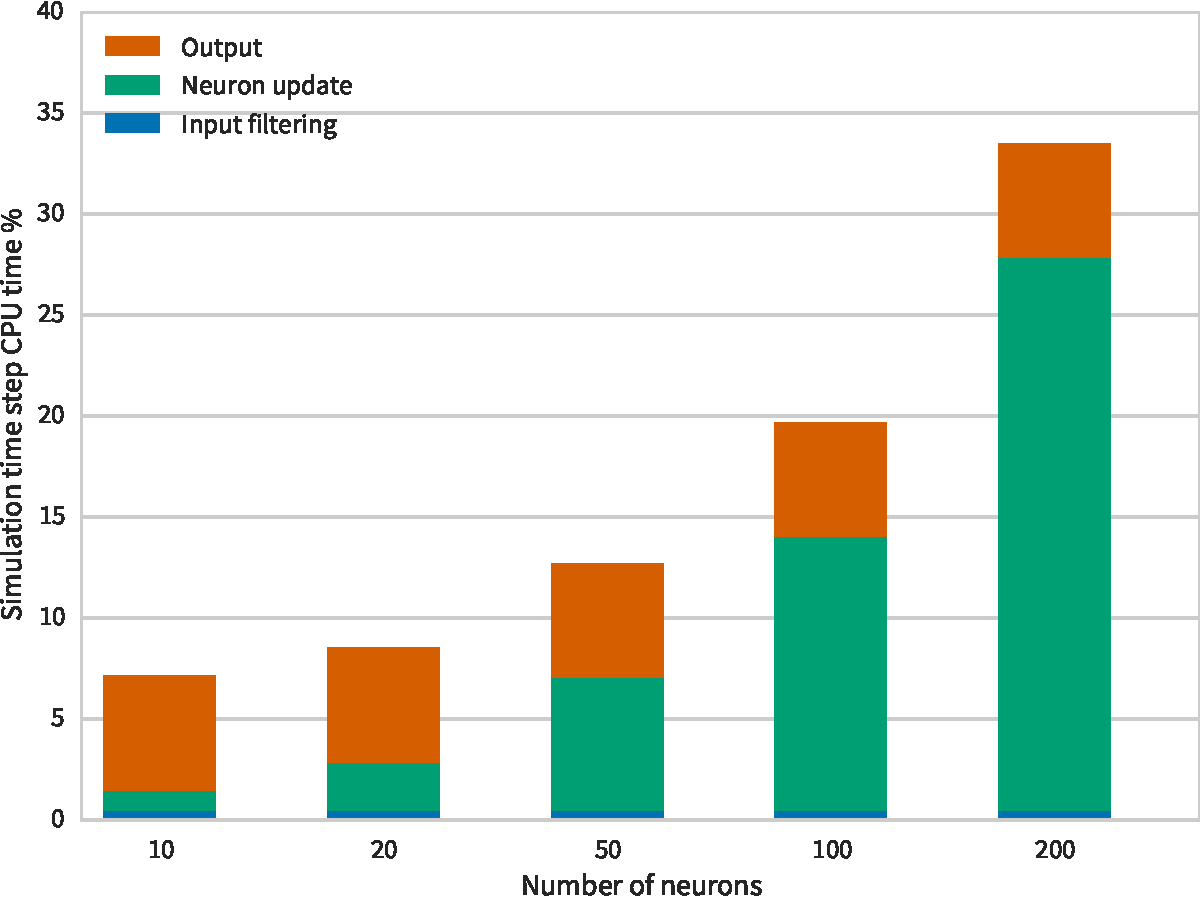
\includegraphics[width=\textwidth]{figures/comm_channel_cpu_16d_bar.pdf}

    {\tiny 16-D representation, \SI{200}{\mega\hertz} clock cycle with
     \SI{1}{\milli\second} simulation step}
  \end{frame}

  \begin{frame}{Results}
    \begin{itemize}
      \item Reduced compute cost scaling -- $0.19N^2$ vs. $3N^2$\\
            (fixing $D = \frac{N}{70}$)
        \begin{itemize}
          \item Up to 2000 neurons per core -- 2x target
        \end{itemize}
      \item Memory usage reduced by \SI{90}{\percent}+
        \begin{itemize}
          \item Also affects load time
        \end{itemize}
    \end{itemize}
  \end{frame}

  % Future Work
  % -----------
  % * Computational effect on learning rules (particularly PES)
  % * Further code improvements
  \begin{frame}{In conclusion}
    NEF on GPU --
    \begin{itemize}
      \item \num{500000} neurons in real-time (Radeon HD7970)
      \item Scaling beyond one GPU may be difficult
      \item Large power consumption
    \end{itemize}

    \vskip\baselineskip

    NEF on other neuromorphic hardware --
    \begin{itemize}
      \item Limited by number of available synapses
      \item \textit{Brainstorm}\footnote{\url{http://brainstorm.stanford.edu/projects/}} designed for the NEF
      \item SpiNNaker is very flexible
    \end{itemize}
  \end{frame}

  \begin{frame}{In conclusion}
    Future work --
    \begin{itemize}
      \item Real-time Spaun
      \item Analyse effect on learning-rules
      \item Analyse effect on network loading
    \end{itemize}
  \end{frame}

  \begin{darkframes}
    \begin{frame}{~}
      \vfill
      \vfill
      {Andrew Mundy\\andrew.mundy@ieee.org}
    \end{frame}
  \end{darkframes}
\end{document}
